\section{Results}

\subsection{Healthcare System Cost Savings}

We quantified the potential long-term savings to healthcare systems based on our modeled intervention strategies derived from DunedinPACE data, comparing these savings against current projections of aging-related healthcare expenditures.

Our analysis revealed significant savings across all intervention scenarios compared to the baseline control (no aging-pace intervention). We constructed two distinct scenarios: Scenario 1 examined a hypothetical cohort followed from age 50 to 90, assuming all individuals remained alive throughout the 40-year period; Scenario 2 incorporated natural mortality patterns, progressively reducing cohort size over time. Notably, our analysis excluded costs associated with the health technology enabling DunedinPACE monitoring and control.

The savings became increasingly pronounced over time as intervention effects accumulated, delaying frailty onset and progression. Under Scenario 1 assumptions, cumulative savings reached CHF 43,675 with the CR0 DunedinPACE control strategy, CHF 112,427 with CR1, and CHF 131,608 with CR2 (Figure~\ref{fig:savings}, left panel).

Scenario 2 demonstrated more complex dynamics. As frailty-related mortality increased with age, robust individuals comprised an increasing proportion of survivors, particularly in intervention scenarios. This created the cumulative savings pattern shown in Figure~\ref{fig:savings} (right panel). Savings peaked at approximately age 85 (35 years post-intervention initiation), with CR2 showing the most pronounced benefits compared to CR1 and CR0. Interestingly, the trend reversed after age 95, eventually resulting in net losses to healthcare systems. This counterintuitive finding reflects the intervention's success in extending lifespan, thereby increasing the proportion of individuals requiring late-life healthcare services—a phenomenon observed in other therapeutic domains, such as oncology, where survival extension often necessitates continued healthcare expenditures.

\begin{figure}[h]
\centering
\small
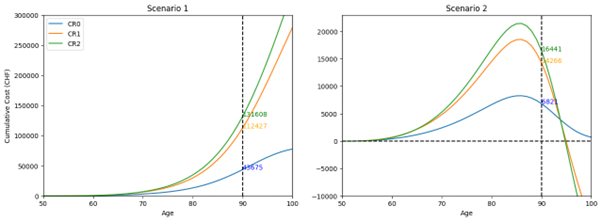
\includegraphics[width=\textwidth]{figures/Figure5.png}
\caption{Cumulative healthcare system costs under two scenarios. Scenario 1 follows a cohort from age 50 to 90 assuming no mortality. Scenario 2 incorporates natural mortality progressively reducing cohort size. Lines show cumulative savings under three epigenetic clock control strategies: CR0 (blue), CR1 (orange), and CR2 (green).}
\label{fig:savings}
\end{figure}

\subsection{Value to Individuals}

While healthcare system savings provide valuable perspective on intervention cost-effectiveness from a payer standpoint, this analysis has limitations. It focuses solely on frailty-related direct costs, omitting costs indirectly linked to frailty (e.g., comorbidities such as dementia, cancer, or cardiovascular disease). Additionally, it extrapolates Dutch healthcare data to the Swiss context, where frailty-related expenditures may differ significantly.

We therefore extended our analysis to quantify individual value, building on the economic framework outlined in the Methods section. We determined lifespan and healthspan changes induced by the three CR regimens, combining these with life-year values $v(t)$ and marginal consumption utility to generate willingness-to-pay curves for the health technology $\xi$.

Survival curves shifted rightward with increasing DunedinPACE control, with effects most pronounced in individuals over 80—those most likely to be frail in the baseline scenario (Figure~\ref{fig:lifespan_healthspan}, top-left panel). The effect magnitude peaked around age 90 (Figure~\ref{fig:lifespan_healthspan}, bottom-left panel). Regarding healthspan, control regimens significantly reduced health-related quality-of-life decline, maintaining high quality-of-life levels throughout aging, with the CR2 scenario even showing slight improvements (Figure~\ref{fig:lifespan_healthspan}, right panels).

\begin{figure}[h]
\centering
\small
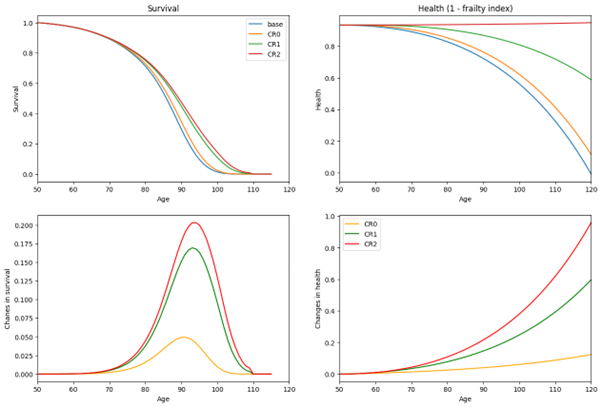
\includegraphics[width=\textwidth]{figures/Figure6.png}
\caption{Lifespan (survival, left column) and healthspan (right column) evolution under three control scenarios. Top row shows baseline evolution (blue) and corresponding curves for CR0 (orange), CR1 (green), and CR2 (red). Bottom row shows changes in survival and health for each control scenario relative to baseline.}
\label{fig:lifespan_healthspan}
\end{figure}

Mean life expectancy was 84.34 years in the baseline scenario, increasing to 85.11 years with CR0, 87.22 years with CR1, and 87.92 years with CR2—representing life expectancy gains ranging from 0.77 to 3.58 years (Table~\ref{tab:lifeexp}).

\begin{table}[h]
\centering
\small
\setlength{\tabcolsep}{5pt}
\begin{tabular}{lrr}
\toprule
\textbf{Scenario} & \textbf{Life expectancy} & \textbf{Life expectancy gain} \\
\midrule
Base & 84.34 & 0.00 \\
CR0 & 85.11 & 0.77 \\
CR1 & 87.22 & 2.89 \\
CR2 & 87.92 & 3.58 \\
\bottomrule
\end{tabular}
\caption{Life expectancy across scenarios and gains relative to baseline.}
\label{tab:lifeexp}
\end{table}

Calculating willingness-to-pay for lifespan and healthspan changes required incorporating profiles of $v(t)$ and marginal consumption utility, calibrated using parameters from Scott et al.~\cite{Scott2023b}. The monetary value $v(t)$ showed a decreasing trend with age (Figure~\ref{fig:value_utility}, left panel), while the marginal consumption utility exhibited a more complex pattern (Figure~\ref{fig:value_utility}, right panel). Notable inflection points occur at age 65 due to retirement: $v(t)$ drops reflecting reduced income, while utility increases sharply, reflecting increased leisure time availability.

\begin{figure}[h]
\centering
\small
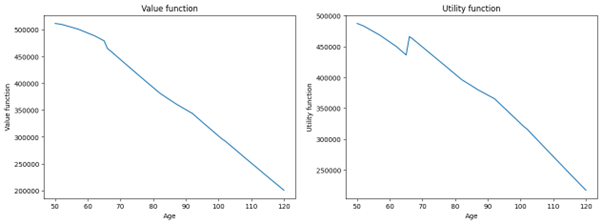
\includegraphics[width=\textwidth]{figures/Figure7.png}
\caption{Value function $v(t)$ (left) and marginal utility function for consumption (right) across age.}
\label{fig:value_utility}
\end{figure}

The CR2 scenario generated the highest willingness-to-pay due to its impact on both lifespan and life quality. Lifestyle changes affecting DunedinPACE yielded highest willingness-to-pay values between ages 80-100, when frailty reduction benefits are most pronounced (Figure~\ref{fig:wtp}, left panels). Health improvements affected willingness-to-pay from earlier ages, with notable increases around age 65 due to retirement-related leisure time valuation (Figure~\ref{fig:wtp}, right panels).

\begin{figure}[h]
\centering
\small
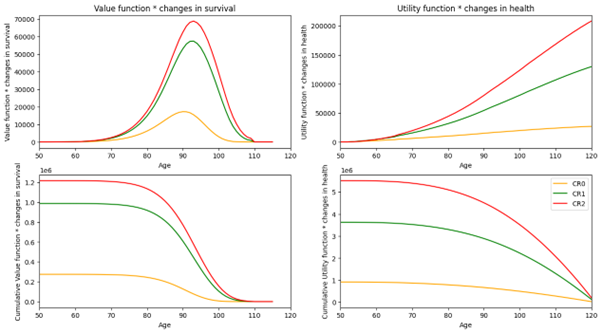
\includegraphics[width=\textwidth]{figures/Figure8.png}
\caption{Annual willingness-to-pay for additional life based on survival changes (top-left) and cumulative willingness-to-pay from age 50 (bottom-left). Annual utility values from health improvements (top-right) and corresponding cumulative utility from age 50 (bottom-right).}
\label{fig:wtp}
\end{figure}

Cumulative willingness-to-pay curves demonstrated substantial valuations for both survival and health changes, exceeding CHF 1.2 million for survival and CHF 5.5 million for health improvements under the strictest DunedinPACE control scenario CR2 (Table~\ref{tab:wtp}). Note that these values are undiscounted, assuming no personal time preference.

\begin{table}[h]
\centering
\small
\setlength{\tabcolsep}{4pt}
\begin{tabular}{lrrr}
\toprule
\textbf{Scenario} & \textbf{Survival Changes} & \textbf{Health Changes} & \textbf{Total Value} \\
\midrule
CR0 & 274.68 & 916.92 & 1,191.59 \\
CR1 & 986.78 & 3,628.88 & 4,615.66 \\
CR2 & 1,216.19 & 5,515.61 & 6,731.80 \\
\bottomrule
\end{tabular}
\caption{Willingness-to-pay at age 50 for changes in survival, health, and their combination over remaining lifespan (thousands of CHF).}
\label{tab:wtp}
\end{table}

\subsection{Squaring the Survival Curve}

"Squaring the survival curve" is a concept in public health and gerontology describing an ideal survival trajectory where individuals remain healthy until very near their life expectancy, followed by a rapid decline~\cite{Caselli2021}. This contrasts with traditional survival curves showing steady decline from birth with accelerating mortality at advanced ages.

The squared curve represents a compression of morbidity scenario—individuals live full, healthy lives with minimal disability or chronic disease until shortly before death, rather than experiencing prolonged periods of diminished health.

Our assessment of DunedinPACE control scenarios demonstrated progressively more rectangular health-versus-survival curves with stricter control regimens. The CR2 strategy in particular produced a more squared curve, suggesting successful morbidity compression and the potential for individuals to maintain high quality of life until near death (Figure~\ref{fig:squaring}).

\begin{figure}[h]
\centering
\small
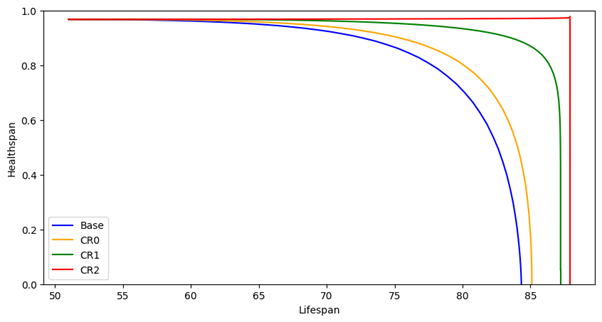
\includegraphics[width=\textwidth]{figures/Figure9.png}
\caption{Squaring the survival curve: healthspan versus lifespan for CR0 (orange), CR1 (green), and CR2 (red) scenarios. Stricter DunedinPACE control produces increasingly rectangular survival curves, indicating compressed morbidity.}
\label{fig:squaring}
\end{figure}

\subsection{Quality-Adjusted Life Year Gains}

Quality-Adjusted Life Years (QALYs) combine quantity and quality of life into a single metric used in health economics to assess intervention value~\cite{Briggs2023}. One QALY represents one year in perfect health.

The Incremental Cost-Effectiveness Ratio (ICER) evaluates new medical interventions by dividing cost difference by QALY difference:

\begin{equation}\label{eq:icer}
ICER = \ \frac{\mathrm{\Delta}_{\xi}Cost}{\mathrm{\Delta}_{\xi}QALY}
\end{equation}

where $\mathrm{\Delta}_{\xi}QALY$ and $\mathrm{\Delta}_{\xi}Cost$ represent QALY and cost changes attributable to health technology $\xi$. Our analysis to this point excluded intervention costs, so ICER calculations will inform pricing strategies for the technology.

ICER thresholds represent maximum willingness-to-pay for one additional QALY. The World Health Organization suggests thresholds of 1-3× GDP per capita~\cite{Woods2016}. With Switzerland's GDP per capita approximating CHF 100,000 (2023-2024)~\cite{IMF}, relevant ICER thresholds range from CHF 100,000-300,000.

Our model calculated QALY gains of 1.07 for CR0, 3.90 for CR1, and 5.32 for CR2. Using these thresholds, willingness-to-pay ranges from approximately CHF 107,000 (CR0, lowest threshold) to over CHF 1.5 million (CR2, highest threshold) (Table~\ref{tab:qaly}).

\begin{table}[h]
\centering
\small
\setlength{\tabcolsep}{3pt}
\begin{tabular}{lrrrr}
\toprule
\textbf{Scenario} & \textbf{QALY} & \textbf{$\mathbf{\Delta}$QALY} & \textbf{ICER} & \textbf{WTP} \\
\midrule
Base & 80.19 & 0.00 & 100,000 & 0 \\
CR0 & 81.26 & 1.07 & 100,000 & 107,173 \\
CR1 & 84.09 & 3.90 & 100,000 & 389,901 \\
CR2 & 85.51 & 5.32 & 100,000 & 531,628 \\
\midrule
Base & 80.19 & 0.00 & 200,000 & 0 \\
CR0 & 81.26 & 1.07 & 200,000 & 214,346 \\
CR1 & 84.09 & 3.90 & 200,000 & 779,803 \\
CR2 & 85.51 & 5.32 & 200,000 & 1,063,257 \\
\midrule
Base & 80.19 & 0.00 & 300,000 & 0 \\
CR0 & 81.26 & 1.07 & 300,000 & 321,519 \\
CR1 & 84.09 & 3.90 & 300,000 & 1,169,704 \\
CR2 & 85.51 & 5.32 & 300,000 & 1,594,885 \\
\bottomrule
\end{tabular}
\caption{QALY gains across intervention scenarios at three ICER threshold levels (CHF 100,000-300,000).}
\label{tab:qaly}
\end{table}

The expected outcomes of the proposed DunedinPACE monitoring and intervention strategy include reduced frailty and chronic disease burden, improved individual health and wellbeing across the lifespan, enhanced healthcare system efficiency, and positive economic and social welfare effects.

Preliminary evidence from our pilot study with 100 Dunedin Study participants demonstrates the feasibility and acceptability of DunedinPACE assessments and personalized interventions. Participants reported high satisfaction and adherence, with improved biomarkers and health outcomes after six months of follow-up, supporting the viability of the proposed approach.
